\chapter{Background}

\section{Exploratory Data Analysis}
There are 124883 out of 125280 sessions which appear only once in the Microsoft dataset.
The dataset can be found in Appendix \ref{tab:headdf} and sessions look like Appendix \ref{lst:sessions}.
If we divide sessions into sequences of commands of length 12\cite{sadique2021analysis},
many sequences seem to be naturally clustered by frequncies of appearance, as shown in Fig \ref{fig:EDA}.
Within each cluster, not only the distribution of initial few commands seem very homogeneous,
but also the sequences themselves.
\begin{figure}[h]
    \centering
    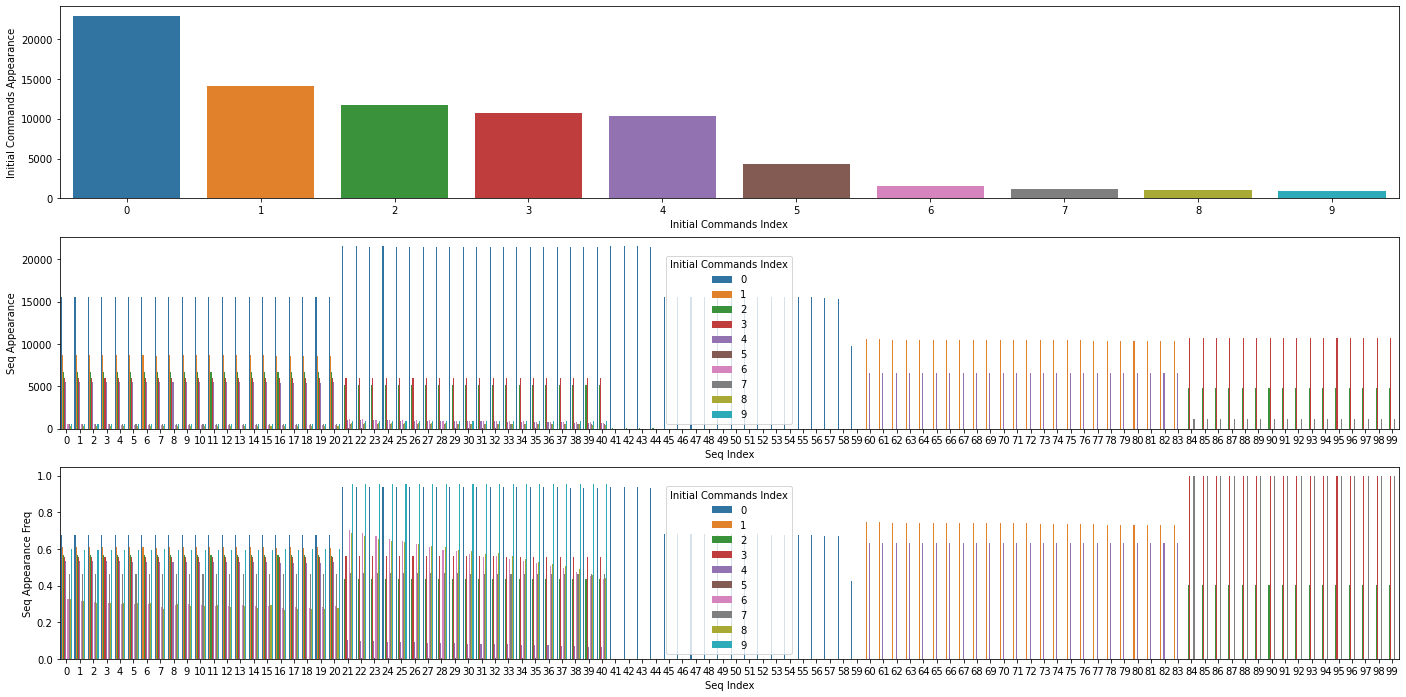
\includegraphics[scale=0.3]{background/EDA.png}
    \caption{Exploratory Data Analysis. The top graph shows the number of appearance of 
    top 10 frequent initial 3 commands. The middle graph shows the number of appearance of 
    top 10 frequent initial 3 commands in sessions which contain top 100 frequent sequence of commands.
    The bottom graph shows the frequency of top 10 frequent 
    initial 3 commands in sessions which contain top 100 frequent sequence of commands}
    \label{fig:EDA}
\end{figure}
\\
This encourages us to try to cluster and predict the commands based on the initial commands in a session.
\section{Data Pre-processing}
There are 3 major objectives in data processing.
\begin{enumerate}
    \item Seperate multiple commands in one command line.
    \item Use \textbf{r'[a-zA-Z0-9\_$\backslash$.$\backslash$-$\backslash$*]+'} as regexp to tokenise commands into words.
    \item Replace the words which only appear in one session by rarecommand.
\end{enumerate}
The sample code can be found in Appendix \ref{lst:tokeniser}
\section{Hierarchical Agglomerative Clustering}
Hierarchical clustering is a method which exhaustively merge pairs of clusters.
Each observation starts in its own cluster. 
Iteratively, the closest (most similar) pairs of clusters merge, 
until there is only one cluster or the threshold is achived.